\documentclass{article}

\usepackage{graphicx}
\usepackage{indentfirst}
\usepackage[a4paper, total={6in, 8in}]{geometry}
\usepackage{hyperref}
\usepackage{fancyhdr}
\usepackage{xepersian}


\usepackage{booktabs}
\settextfont{B Nazanin}
\setlatintextfont{Times New Roman}
\renewcommand{\labelitemi}{$\bullet$}
\renewcommand{\labelitemii}{$\bullet$}

\begin{document}


%title page%
\begin{titlepage}
	\begin{center}
		\vspace{0.2cm}
		
		
\includegraphics[width=0.4\textwidth]{sharif.png}\\
		\vspace{0.2cm}
		\textbf{ \Huge{آزمایش شماره 1}}\\
		\vspace{0.25cm}
		\textbf{ \Large{آز شبکه - دکتر بردیا صفایی}}
		\vspace{0.2cm}
		
		
		\large \textbf{دانشکده مهندسی کامپیوتر}\\\vspace{0.1cm}
		\large   دانشگاه صنعتی شریف\\\vspace{0.2cm}
		\large   ﻧﯿﻢ‌سال اول ۰۱-۰۲ \\\vspace{0.10cm}
		\large{\href{mailto:mehrshad.mirmohammadi@gmail.com}{مهرشاد میرمحمدی - 98109634}}\\
		\large{\href{mailto:parhaamsaremi@gmail.com}{پرهام صارمی - 97101959}}\\
		\large{\href{mailto:mofayezi.m@gmail.com}{محمدرضا مفیضی - 98106059}}\\
	\end{center}
\end{titlepage}
%title page%

\newpage

%pages header
\pagestyle{fancy}
\fancyhf{}
\fancyfoot{}
\setlength{\headheight}{59pt}
\cfoot{\thepage}
\lhead{آزمایش شماره ۱}
\rhead{
\includegraphics[width=0.1\textwidth]{sharif.png}\\
		دانشکده مهندسی کامپیوتر
}
\chead{آز شبکه}
%pages header

\section{کابل‌ها}
%در جدول زیر مقایسه عددی سه کابل \lr{coaxial} و \lr{twisted pair} و فیبر نوری آمده است:
%\begin{table}[h]
%	\centering
%	\begin{tabular}{r|c|c|c}
%		نوع کابل & حداکثر سرعت انتقال داده & احتمال ایجاد خطا & حداکثر مسافت طی‌شده \\
%		\hline
%		کابل \lr{coaxial} & 80 گیگابیت بر ثانیه  & 750 مگاهرتز & 500 متر \\
%		\hline
%		کابل \lr{twisted pair} & 10 گیگابیت بر ثانیه & 4700 مگاهرتز & 100 متر \\
%		\hline
%		فیبر نوری & 200 گیگابیت بر ثانیه & 4700 مگاهرتز & 80 کیلومتر \\
%		\end{tabular}
%	\caption{مقایسه عددی سه کابل}
%	\label{tab:cable_comp}
%\end{table}

سرعت انتقال داده در فیبر نوری از بقیه بیشتر و سپس کابل \lr{coaxial} و درانتها \lr{twisted pair} قرار دارد.

از لجاظ احتمال ایجاد خطا، کابل \lr{twisted pair} بدترین عملکرد را دارد سپس کابل \lr{coaxial} به دلیل وجود هادی محافظ مقاومت بیش‌تری دربرابر نویز دارد و به دلیل بی‌اثر بودن نویز الکتریکی بر نور، فیبر نوری کم‌ترین احتمال ایجاد خطا را دارد.

فیبر نوری کمترین میزان کاهش انرژی سیگنال سپس کابل \lr{coaxial} و درانتها \lr{twisted pair} قرار دارد.

کابل \lr{twisted pair} نصب آسان و ارزان‌تری نسبت به بقیه دارد. کابل \lr{coaxial} نیز نصب آسانی دارد اما هزینه بیش‌تری نسبت به \lr{twisted pair} دارد. نصب فیبر نوری از بقیه سخت‌تر و هزینه آن نیز بیش‌تر است. بنابراین زمانی که سرعت بالا و خطای پایین اهمیت دارد استفاده از فیبر نوری توجیه‌پذیر است و درغیراین صورت دو کابل دیگر باتوجه به هزینه پایین‌تر مقرون‌به‌صرفه هستند.

\section{معماری \lr{TCP/IP}}
معماری \lr{TCP/IP} یا همان \lr{Transmission Control Protocol/Internet Protocol} مجموعه‌ای از پروتکل‌های ارتباطی است که برای اتصال دستگاه‌ها در شبکه اینترنت استفاده می‌شود.
پروتکل های اصلی فعلی در این مجموعه عبارتند از پروتکل کنترل انتقال (\lr{TCP}) و پروتکل اینترنت (\lr{IP})، و همچنین پروتکل \lr{UDP} است.

مجموعه پروتکل \lr{IP}، ارتباط \lr{end-to-end} داده‌ها را فراهم می‌کند که مشخص می‌کند چگونه داده‌ها باید دسته‌بندی، آدرس‌دهی، منتقل، مسیریابی و دریافت شوند.
این قابلیت در چهار لایه انتزاعی سازماندهی شده است که تمام پروتکل‌های مرتبط را بر اساس محدوده شبکه هر پروتکل طبقه‌بندی می‌کند. لایه‌ها از پایین به بالا به ترتیب:
\begin{enumerate}
	\item
	  لایه لینک \LTRfootnote{\lr{link}} که شامل روش‌های ارتباطی برای داده‌هایی هست که در یک سگمنت از شبکه باقی می‌مانند. 
	\item 
	لایه اینترنت \LTRfootnote{\lr{internet}} با بسته‌ها سر و کار دارد و شبکه‌های مستقل را برای انتقال بسته‌ها از مرزهای شبکه به هم متصل می‌کند. پروتکل‌های لایه شبکه پروتکل \lr{IP} و پروتکل کنترل پیام اینترنت \LTRfootnote{\lr{ICMP}} هستند که برای گزارش خطا استفاده می‌شوند. 
	\item
	لایه انتقال \LTRfootnote{\lr{transport}} وظیفه حفظ ارتباطات \lr{end-to-end} شبکه را بر عهده دارد. \lr{TCP} ارتباطات بین میزبان‌ها را مدیریت می‌کند و کنترل جریان \LTRfootnote{\lr{flow control}}، \lr{multiplexing} و \lr{reliability} را فراهم می‌کند. پروتکل‌های لایه انتقال شامل \lr{TCP} و \lr{UDP} است. 
	\item
	در نهایت لایه کاربرد \LTRfootnote{\lr{application}} تبادل داده استاندارد‌شده را برای برنامه‌ها پیاده‌سازی می‌کند. \lr{FTP} و \lr{HTTP} دو نمونه از پروتکل‌های این لایه هستند. در لایه کاربرد، \lr{payload}، داده واقعی برنامه است.
\end{enumerate}

تفاوت اصلی بین دو معماری \lr{TCP/IP} و \lr{OSI} این است که \lr{OSI} یک مدل مفهومی است که عملا در شبکه استفاده نمی‌شود. در عوض، نحوه ارتباط برنامه‌ها از طریق شبکه را مشخص می‌کند. از طرف دیگر، \lr{TCP/IP} به طور گسترده برای ایجاد لینک‌ها و ارتباطات شبکه استفاده می‌شود.
پروتکل‌های \lr{TCP/IP} استانداردهایی را ارائه می‌کنند که اینترنت بر اساس آن ایجاد شده است، در حالی که مدل \lr{OSI} دستورالعمل‌هایی را در مورد نحوه برقراری ارتباط ارائه می‌کند. بنابراین، \lr{TCP/IP} یک مدل کاربردی‌تر است.

مدل های \lr{TCP/IP} و \lr{OSI} شباهت‌ها و تفاوت‌هایی دارند. شباهت اصلی در ساختار آنهاست به که هردو به صورت لایه‌ای است، اگرچه \lr{TCP/IP} فقط از چهار لایه تشکیل شده است اما مدل \lr{OSI} دارد.
از دیگر تفاوت‌های این دو مدل این است که معماری \lr{TCP/IP} از یک لایه کاربرد برای تعریف عملکرد لایه‌هایی بالایی استفاده می‌کند، درحالی که معماری \lr{OSI} از سه لایه کاربرد، نمایش و نشست استفاده می‌کند. در \lr{TCP/IP} اندازه هدر \LTRfootnote{\lr{header}} 20 بایت ولی در \lr{OSI} 5 بایت است. 

همچنین از لحاظ تاریخی در \lr{TCP/IP} اول پروتکل‌ها طراحی شدند سپس مدل به وجود آمد اما در \lr{OSI} ابتدا مدل طراحی شد و سپس پروتکل‌های هرلایه طراحی شدند.

\newpage

در شکل \ref{fig:layers} نمای کلی لایه‌های دو معماری نمایش داده شده است. 
\begin{figure}[h]
	\centering
	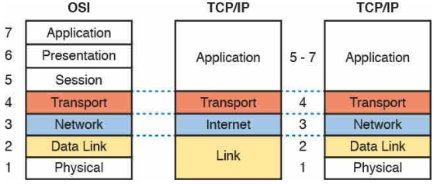
\includegraphics[width=0.6\columnwidth]{figs/osi-tcpip.jpg}
	\caption{لایه‌های معماری \lr{TCP/IP} و \lr{OSI}}
	\label{fig:layers}
\end{figure}

\section{استاندارد \lr{straight} و \lr{cross}}
از کابل‌های \lr{straight} برای اتصال دو نوع دستگاه متفاوت و از استاندارد \lr{cross} برای اتصال دو دستگاه از یک نوع استفاده می‌شود.

استاندارد اترنت \LTRfootnote{\lr{Ethernet}} قراردادهای اتصال کابل‌ها را تعریف می‌کند که به عنوان مثال \lr{100BASE-TX} و \lr{1000BASE-T} دو نمونه از آن‌ها هستند. این دو استاندارد از 4 جفت کابل \lr{twisted pair} استفاده می‌کنند که دوتای آن‌ها یعنی جقت 2 و 3 برای ارسال و دریافت اطلاعات استفاده می‌شوند.
 در هر \lr{PC} ارسال اطلاعات همیشه روی جفت 2 و دریافت روی جفت 3 انجام می‌شود. بنابراین اگر دو \lr{PC} مستقیما به هم وصل شوند هردو روی جفت 2 داده ارسال می‌کنند. پس در این حالت باید از استاندارد \lr{cross} برای اتصال استفاده شود تا تداخل پیش نیاید.
 
 در سوئیچ‌ها ارسال اطلاعات از طریق جفت 2 و دریافت از طریق جفت 3 انجام می‌شود (به صورت ضمنی یک \lr{crossover} داخلی ایحاد می‌شود). بنابراین در اتصال یک \lr{PC} به یک سوئیچ می‌توان از روش \lr{straight} استفاده کرد و بدون آن که مشکلی برای دریافت‌کننده و فرستنده اطلاعات ایجاد شود.
 واضح است که برای اتصال دو سوئیچ، برای جلوگیری از تداخل باید از روش \lr{cross} استفاده شود.
 در یک \lr{Router} مانند یک \lr{PC} ارسال روی جفت 2 و دریافت روی جفت 3 انجام می‌شود و در هاب‌ها مشابه سوئیچ‌ها ارسال روی 3 و دریافت روی 2 انجام می‌شود.
 
 به صورت خلاصه برای اتصال یک سوئیچ یا هاب به سوئیچ یا هاب دیگر از روش \lr{cross}، برای اتصال یک سوئیچ یا هاب به یک \lr{PC} یا \lr{Router} از روش \lr{straight} و برای اتصال دو \lr{PC} یا \lr{Router} به هم از روش \lr{cross} استفاده می‌شود.
 بنابراین در دنیای امروزی کابل‌های \lr{straight} (در حالت‌های گفته شده) بدون مشکل مورد استفاده قرار می‌گیرند.

\end{document}
